
%Speakers exhibit considerable production variability at all levels 
%of linguistic representation \egcite{Liberman1967, Weiner1983,Finegan2001}. This includes 
%variation in lexical choice to describe a world state. For example, \cite{Yildirim2016} found that 
%when asked to describe a scene with a candy bowl in which approximately half of the candies were green
%and half of the candies were blue, some participants judged ``Some of the candies are green'' to be the more appropriate
%utterance to describe the scene than ``Many of the candies are green'', while others displayed the opposite pattern. 


%\cite{Schuster2018} found that participants exhibit similar production variability when describing 
%an event with an objective event probability of 60\%: Some participants judged the event to be
%best described with a sentence containing the uncertainty expression \textit{might} (``You might get a blue gumball'') 
%whereas others judged a sentence with \textit{probably} (``You'll probably get a blue gumball'') more
%appropriate.

%Such variability poses a challenge to a listener who aims to know what the world is like that the speaker is describing. 
%When confronted with two speakers who use the same expression to convey different states of the world or
%who use different expressions to convey the same state of the world, listeners are doomed to draw the 
%wrong inferences about the actual state of the world unless they track how individual speakers use language.%
%Recent work suggests that listeners deal with this kind of variability by adapting to it 
%\egcite{Norris2003,Kraljic2007,Bradlow2008, Kamide2012,Kleinschmidt2015,Fine2016,Roettger2019} and 
%that in interaction, they learn how speakers choose among alternative 
%utterances. In the domain of quantifiers,  
%\textcite{Yildirim2016} showed that listeners update their expectations about how a specific speaker uses the quantifiers 
%\textit{some} or \textit{many} after being briefly exposed to a specific speaker. 

In the previous chapter, I found that listeners update their expectations of how a specific speaker
uses the uncertainty expressions \textit{might} and \textit{probably} to describe different event probabilities after a brief
exposure phase. Participants who were exposed to the ``\textit{confident}'' speaker, who used \textit{probably} to describe the 60\% probability event, 
 expected the use of \textit{probably} with a wider range of probabilities; participants who were exposed to the ``\textit{cautious}'' speaker, who
used \textit{might} to describe the 60\% probability event, expected the use of \textit{might} with a wider range of probabilities.


However, from the results in the previous chapter and other work on semantic adaptation, 
it remains a largely open question to what extent listeners form speaker-specific
expectations when interacting with multiple speakers. Some evidence for speaker-specific
adaptation comes from the referring expressions literature. As I discussed in Chapter~2,  \textcite{Metzing2003} found that 
participants exhibited a slowdown in resolving referring expressions
when a confederate started referring to an object with a new expression 
after establishing a conceptual pact, but did not find such a slowdown 
when a new confederate was using a different referring expression 
than the original confederate. 

Most closely related to my work, \textcite{Yildirim2016} found that listeners 
form speaker-specific production expectations after being exposed to 
two speakers who used different 
quantifiers to describe a scene with a candy bowl
in which half of the candies were green. While this suggests
that listeners should also form speaker-specific expectations
about the use of uncertainty expressions, there is evidence from
other linguistic domains that speaker-specific adaptation is limited to specific items.
For example, \textcite{Kraljic2007} found that listeners adjust their phonemic
representations for the fricatives /s/ and /sh/ to multiple speakers whereas listeners
adjusted their phonetic representations for stop consonants such as /d/ and /t/ only
to the most recent conversational partner. It could therefore be that speaker-specific adaptation
in other linguistic domains is also limited to specific items and that listeners do not
form speaker-specific expectations for the use of uncertainty expressions.

Further, \textcite{Yildirim2016} observed that the adaptation effect was considerably smaller
when they exposed participants to two speakers with opposing biases as compared 
to only exposing participants to one speaker and comparing the adaptation 
effect between groups. There seem to be two likely explanations for this observation.
First, it could be that due to memory limitations, listeners were unable 
to keep track of the exact statistics of each speaker's utterances. Since
everything about the context except the speaker identity stayed constant
throughout the experiment, it could be that listeners had difficulty 
separating their experiences with the two speakers in memory (see \textcite{Horton2005} for 
a similar account of memory limitations affecting audience design). Second, it
could be that listeners were tracking the statistics of the individual speakers as
well as the overall statistics in the experimental situation and their post-exposure
expectations were a combination of their speaker-specific expectations as well as 
their expectations about the situation.

In this chapter, I take a first step towards investigating the nature of semantic adaptation 
in response to multiple speakers. 
In particular,
I aim to answer the following two questions:
\begin{enumerate}
    \item Do listeners form speaker-specific production expectations when they are 
             exposed to speakers whose use of uncertainty expressions differ? 
    \item Do listeners form situation-specific production expectations independent of speaker identity?
\end{enumerate}    

In Experiment 4, I address question 1 by exposing listeners to two
speakers whose use of uncertainty expressions differs. In Experiment 5, I expose listeners to two speakers whose use of uncertainty expressions is the same. I compare adaptation effect sizes across experiments to address question 2.

\section{Experiment 4: Different speaker types}

In both experiments, I use the same exposure-test paradigm as in the previous chapters, including the same types of recordings.
In Experiment 4, I exposed participants to two different speakers who 
use the uncertainty expressions \textit{might} and \textit{probably} differently. 
The primary purpose of this experiment was to test whether listeners  
form speaker-specific  utterance choice expectations.
Procedure, materials, analyses and exclusions
were pre-registered on OSF (https://osf.io/qnspg).

\subsection{Methods}

\paragraph{Participants}
 I recruited 104 participants on Amazon Mechanical Turk. 
Participants had to have a US-based IP address and a minimal approval rating of 
95\%, and they were paid \$4.75 (approximately \$12--\$15/hr). 

\paragraph{Materials and procedure}

 In the first part of the experiment, participants saw 40 exposure trials in two blocks. As in the previous experiments,  each trial showed a child requesting a blue or orange gumball, a gumball machine with blue and orange gumballs, and a video of an adult male or female speaker. The speaker always produced one of the following six utterances:%\vspace{5pt}
 
%\noindent %$\bullet$ 
\begin{itemize}
\item You'll get a blue/orange one (\textsc{bare})
\item You might get a blue/orange one (\textsc{might})
\item You'll probably get a blue/orange one (\textsc{probably})
\end{itemize}

%\vspace{5pt}

The number of trials with each of these utterances as well as the gumball proportions varied across the two blocks (see Table \ref{tab:materials} for an overview). Filler trials with the bare form were included to provide evidence that the speaker is generally cooperative. One of the blocks always showed a female speaker and the other block always showed a male speaker. The order of blocks and the speaker assignment to blocks was counterbalanced across participants. 

\begin{table}
\centering
\begin{tabular}{l c c c c c c}
\toprule
& \multicolumn{2}{c}{\sc might} & \multicolumn{2}{c}{\sc probably} & \multicolumn{2}{c}{\sc bare}\\
& $n$ & $p$ & $n$ & $p$ & $n$ & $p$\\
\midrule
cautious & {\bf 10} & {\bf 60\%} & 5 & 90\% & 5 & 100\%\\
confident & 5 & 25\% & {\bf 10}  & {\bf 60\%} & 5  & 100\%\\  
\bottomrule
\end{tabular}
\caption{Number of exposure trials ($n$) per utterance ({\sc might}, {\sc probably}, {\sc bare}) and associated proportion of target gumballs ($p$) in the cautious vs.~confident speaker block. Critical trials bolded. \label{tab:materials}}

\end{table}

Participants were instructed to watch what the speaker had to say to the child. The video started automatically after a 400ms delay and participants had the option to replay the video as often as they wanted. To advance, participants had to press a button which was disabled until the video had ended.

 After the two exposure blocks, participants went through two test blocks, in which they saw a picture of one of the two speakers with a gumball machine next to it, and again, a child requesting a blue or an orange gumball. Participants were asked to provide ratings for the responses \textsc{might} and \textsc{probably} as well as the blanked \textit{something else} option by distributing 100 points.   In each block, participants provided ratings for scenes with 9 different gumball machines ranging from 0\% to 100\% blue gumballs. For each machine, participants provided four ratings in total, resulting in 36 trials per block. The order of blocks was counterbalanced such that half of the participants saw them in the same order as the exposure blocks whereas the other half saw them in opposite order.

\noindent \textbf{Attention checks}  To verify that participants were paying attention to the video and the scenes, I included 14 attention checks: after 14 of the exposure trials, participants were shown two different gumball machines and were asked to choose the one they saw on the previous trial. 

\noindent \textbf{Exclusions} I excluded participants who provided correct responses to fewer than 11 attention checks. Based on this criterion, I excluded 31 participants. I further excluded participants whose utterance ratings for the different event probabilities strongly correlated ($R^2 > 0.75$) with their mean utterance ratings across all event probabilities. This suggests that they provided approximately the same ratings independent of the observed scenes and indicates that they did not pay attention. This led to one additional exclusion. None of the results discussed below depend on these exclusions.

\noindent \textbf{Analysis and predictions} 
As in the previous experiments, we expect a more confident speaker uses {\sc probably} for a larger and {\sc might} 
for a smaller range of gumball proportions than a more cautious speaker. I again quantify this prediction by 
fitting a spline with four knots for each 
expression and each participant and computing the area under the curve (AUC) for the splines 
corresponding to each expression, block and participant. 
I test whether listeners update their expectations by computing the difference between 
the AUC of the spline for {\sc might} and of the spline for {\sc probably} for each test block for each 
participant. 

Based on the results of the adaptation experiment with multiple speakers by \textcite{Yildirim2016},
I expect speaker-specific adaptation effects. I therefore predict that the mean AUC difference
will be bigger for the \emph{cautious} speaker test blocks than for the \emph{confident} speaker test blocks.

As a secondary analysis, I also investigate whether the order of exposure blocks 
(\textit{confident} or \textit{cautious} first), the assignment of speaker to speaker type 
(whether the male speaker was the \textit{cautious} speaker or vice versa), or the order 
of the test blocks (same as exposure or reverse) has an effect on adaptation. 
I do not expect any of these factors to have an effect on adaptation.



\subsection{Results and discussion}

Figure~\ref{fig:exp1-results} shows the mean utterance ratings of participants grouped by the two post-exposure test blocks. 
As this plot shows, participants expected the \textit{confident} speaker to be more likely to use \textit{probably} for lower 
event probabilities than the \textit{cautious} speaker. This is also reflected in the AUC differences between the splines for 
{\sc might} and of the splines for {\sc probably}: As predicted, this difference was greater for the  \emph{cautious }speaker 
ratings than for the \emph{confident} speaker ratings ($t(142)=2.92, p < 0.01$).

For my secondary analysis, I fit a linear regression model to predict the AUC difference with speaker type, exposure block order, speaker assignment, and test block order as predictors. Only speaker type is a significant predictor in this model (exposure block order: $\beta=5.72, \ t(139)=1.30, \ n.s.$; speaker assignment: $\beta=1.21, \ t(139)=0.28, \ n.s.$; test block order:  $\beta=2.28, \ t(139)=0.52, \ n.s.$). Further, a model that includes these four predictors does not explain significantly more variance than a model that only includes speaker type as a predictor ($F(3,139)=0.67, \  n.s.$).

\begin{figure}
\center
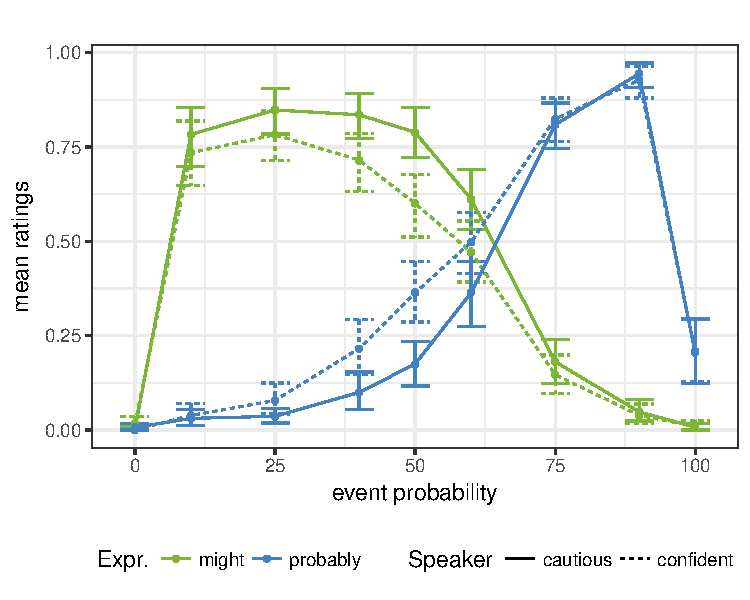
\includegraphics[width=0.5\columnwidth]{plots/exp1-results.pdf}
\caption{Mean utterance ratings for scenes with different event probabilities in Experiment 4. Error bars indicate bootstrapped 95\% confidence intervals. \label{fig:exp1-results}}
\end{figure}

The results of this experiment suggest that listeners form speaker-specific expectations 
of how different speakers use uncertainty expressions after brief exposure. At the same time, the results provide
concrete evidence against two other explanations. First, they provide evidence against an explanation
according to which participants only adapt to the experimental situation: If participants had only updated 
their expectations of what a generic speaker would say in the scenes presented
in the experiment, we would not have expected to see differences in ratings between speakers. Second, they also 
provide evidence against a pure priming account according to which listeners update their expectations to the most 
recent exposure. Note that the adaptation effect was independent of the order of presentation 
and the order of test blocks. If participants had been primed by the most recent exposure speaker, we would have
expected that participants' post-exposure ratings were primarily influenced by the behavior of the second exposure speaker.


The results of this experiment also replicate the 
finding by \cite{Yildirim2016} of differing effect sizes between the single-speaker and
two-speaker experiments: The adaptation effect
was considerably smaller in this two-speaker experiment (Cohen's $d$: 0.486) than in 
the single-speaker adaptation experiment in Chapter~3 (Cohen's $d$: 1.263). 

As suggested by a reviewer, one reason for the smaller effect size in the two-speaker
experiment could be some form of self-priming and that participants' responses in the first 
test block influenced their responses in the second block. I evaluated this hypothesis
in a post-hoc analysis of the responses from the first test block. I 
compared the responses of participants who were first
tested on the \textit{cautious} speaker to the responses of participants who were first tested 
on the \textit{confident} speaker. If responses in the first test block influenced responses in 
the second test block, we would expect a larger effect size if we only consider the data
from the first block. I did indeed find a larger effect size in the first block (Cohen's $d$: 0.723), which
suggests that participants exhibited some form of self-priming.


However, even if we only consider the first block of responses, the adaptation effect 
remains smaller in the two-speaker experiment (Cohen's $d$: 0.723) than in the
one-speaker experiment (Cohen's $d$: 1.263). This could be either a result of memory limitations 
or a result of listeners jointly tracking the statistics of each speaker
as well as of the overall experimental situation (situation-specific statistics).
I further investigate these possibilities in the next experiment.


\section{Experiment 5: Identical speaker types}

In Exp.~4, I found that the adaptation effect was smaller than it was in the single-speaker version of the experiment,
which could have either been a result of memory limitations or joint speaker-specific and situation-specific adaptation. 
In this experiment, I investigate
whether there is evidence for one of these two accounts. I 
exposed listeners to two speakers of the same type.\footnote{
In the spirit of open science, I note that the data from this 
experiment comes from a faulty version of Experiment 4. 
A scripting error led to  participants always being exposed to the 
same speaker type instead of two different speaker types. Because 
of this error, the pre-registered analysis (https://osf.io/3cw79) 
deviates from the analysis that we report here. The reported analyses 
here are the only additional analyses I performed on the data. The 
reason for not discarding the data from this experiment but rather including 
it here is that it provides  an informative data point for the question of whether
listeners track situation-specific expectations.
}
If the smaller effect in Exp.~4 was caused by listeners' inability to separate their experiences with the two speakers in memory, i.e, some experiences might have been attributed to the incorrect speaker, we would expect the adaptation effect in this experiment to be on average the same as in the one-speaker experiment. This is because even if listeners cannot perfectly separate their experiences with each speaker, they would on average still have the same number of experiences with each of the two speakers as listeners had with the one speaker in the single-speaker experiment. If, on the other hand, the smaller effect in the previous experiment was a result of listeners jointly tracking speaker-specific and situation-specific statistics, we would expect the adaptation effect to be larger here than in the single-speaker experiment. This is based on the assumption that more exposures lead to a larger adaptation effect and thus listeners' should adapt more to the situation if they are exposed to two speakers and hence also twice the number of interactions.

\subsection{Methods}

\noindent \textbf{Participants} I recruited 104 participants on Amazon Mechanical Turk. 
Participants had to have a US-based IP address and a minimal approval rating of 
95\%, and they were paid \$5 (approximately \$12--\$15/hr).  

\noindent \textbf{Materials and procedure} The materials and procedures were the same as in Exp.~4 except for the following two modifications.
First, the speaker types for each participant were identical across the two exposure blocks: both speakers were either \textit{confident} or \textit{cautious} speakers.
Second, the number of trials with \textsc{probably} and the number of trials with \textsc{might} were the same (10 trials per utterance and block) whereas in Experiment 4, the \textit{confident} speaker
 produced only 5 instances of \textsc{might} and the \textit{cautious} speaker produced  only 5 instances of \textsc{probably}.\footnote{The reason for the second modification is the above mentioned scripting error. See below for a discussion of potential implications.} Assignment of speaker types was counterbalanced across participants, which means this experiment had a between-subjects manipulation.

  
As in Experiment 4, I excluded participants who provided correct responses to less than 11 of the attention checks as well as participants who seemed to provide random responses as defined above. In total, we excluded 11 participants because of the attention check criterion and 1 more participant because of random responses. 


\noindent \textbf{Analysis and predictions} 
As the primary analysis, I compare the AUC differences between the splines for 
{\sc might} and of the splines for {\sc probably} between participants in the two conditions.
Analogous to Experiment 4, I predict that the mean AUC difference
will be bigger in the \emph{cautious} speaker condition than in the \emph{confident} speaker condition.

I again also investigate whether the assignment of speaker to speaker type or the order 
of the test blocks have an effect on the AUC difference. I do not expect either of these factors
to affect adaptation.

Lastly, I compute the effect size measured by Cohen's $d$. As explained above, I expect
the effect size either to be the same as in the single-speaker experiment or to be larger. 


\subsection{Results and discussion}

\begin{figure}
\center
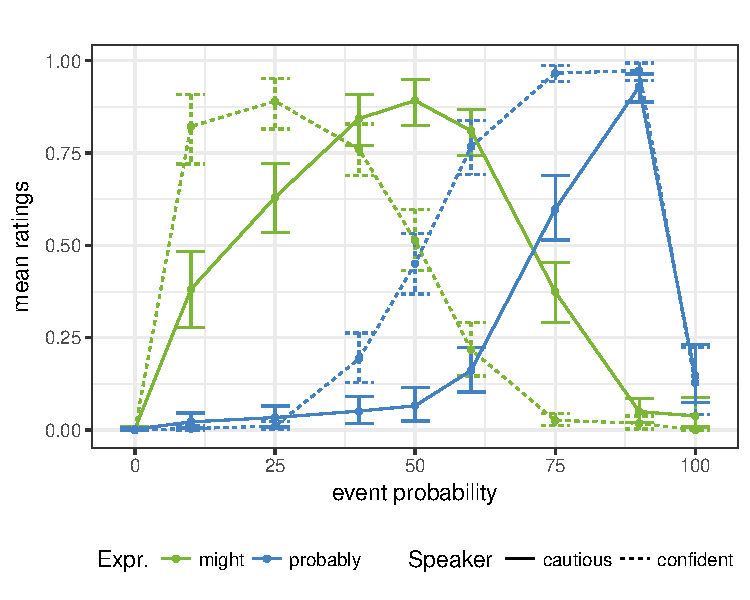
\includegraphics[width=0.5\columnwidth]{plots/exp2-results.pdf}
\caption{Mean utterance ratings for scenes with different event probabilities in Experiment 5. Error bars indicate bootstrapped 95\% confidence intervals. \label{fig:exp2-results}}
\end{figure}

Figure~\ref{fig:exp2-results} shows the mean utterance ratings of participants for the two conditions. We again observe listener adaptation, resulting in a greater AUC difference in the \emph{cautious} speaker 
condition than in the \emph{confident} speaker condition ($t(89)=8.01, p < 0.001$). Further, no factors
other than speaker type are significant predictors of the AUC difference 
(speaker assignment: $\beta=-1.32, \ t(87)=-0.398, \ n.s.$; test block order:  $\beta=4.28, \ t(139)=1.30, \ n.s.$).

Lastly, the effect size (Cohen's $d$: 1.68) was larger in this experiment than in Experiment 4 and the single-speaker 
experiment by \cite{Schuster2018}. While it would be premature to definitively conclude from these three experiments that listeners' expectations are jointly influenced
by individual speaker's productions as well as all the productions in the experiment, our results point in this direction. 

There is a potential confound in this experiment because participants saw 5 additional filler trials during each exposure block which could have led to the larger effect size as compared
to the single-speaker experiment. However, this explanation seems unlikely considering previous work.\footnote{\textcite{Yildirim2016} used 
a very similar paradigm to study semantic adaptation to the use of the quantifiers \textit{some} and \textit{many}. Analagous to our \textit{confident} and 
\textit{cautious} speakers, they had a \textit{some-biased} and a \textit{many-biased} speaker. They report two versions of their experiment: one in which
there were no filler trials with the other quantifier and another version in which there was a balanced number of exposure trials with both quantifiers in both conditions. They found that the adaptation effect was smaller when there were more filler trials, so we would expect that if the additional fillers affected the size of the adaptation effect, the effect would be even larger had we not presented the extra fillers to participants.}


\section{General discussion and conclusion}

In two experiments, we found that listeners form speaker-specific production expectations of 
uncertainty expressions after brief exposure to two speakers. This shows that the results
by \textcite{Yildirim2016} also extend to lexical items other than quantifiers. 

At the same time, however, we found that the adaptation effect size varied depending on 
whether the two speakers had the same or divergent bias during the exposure phase.
When listeners were exposed to two different speaker types, the adaptation effect was smaller
and their expectations seemed to have been shaped by their experiences with the two speakers as well as all the experiences encountered in the experiment.
When both speakers behaved the same, on the other hand, the adaptation effect was much 
more pronounced and even greater than in the single-speaker experiment from previous work.

One likely explanation for these observations is that apart from tracking speaker-specific statistics,
listeners also track the situation-specific statistics of all interactions in the experiment and their expectations
are guided by both of these factors. In the case of speakers with different uses of uncertainty expressions,
speaker-specific adaptation is attenuated since the overall statistics guide listeners towards an ``average''
speaker whose use falls somewhere in between the \textit{cautious} and the \textit{confident} speaker. When listeners
are exposed to two speakers of the same type, on the other hand, the situation-specific statistics reinforce
the speaker-specific statistics and hence listeners adapt more to the two speakers. 

An account based on ``faulty'' memory, according to which listeners have trouble keeping the 
speaker-specific experiences separate, does not predict the larger adaptation effect
when listeners are exposed to two speakers of the same type. If every experience
is encoded as an episode in memory but some with the incorrect speaker information, on average,
the number of experiences with each speaker should still be the same as in the one-speaker
condition and therefore it is unclear why listeners adapt more in the two-speaker experiment than
in the one-speaker experiment.

Our findings also have implications for current models of semantic adaptation. Following the recent
successes in modeling phonetic adaptation as an instance of Bayesian belief updating \cite{Kleinschmidt2015},
\textcite{Schuster2018} propose a computational model of semantic adaptation. According to this model, when interacting with a speaker 
$Sp$, listeners update their beliefs about a set of speaker-specific parameters $\Theta_{Sp}$, which govern the speaker's lexicon and preferences.\footnote{See 
also \cite{Hawkins2017} for a similar model of the formation of conceptual pacts.} 
Their model predicted the results of the single-speaker experiment well, but without modifications, it does not
predict the differences in effect size.

We consider two promising extensions of this model. First, the model could be cast  as a hierarchical model. 
Hierarchical models
have been argued to explain many cognitive and perceptual phenomena \parencite[see, e.g., ][for a review]{Clark2013}, including
phonetic adaptation \cite{Kleinschmidt2019}, and also seem applicable here. 
In a hierarchical version of the adaptation model, we would assume
that the speaker-specific parameters $\Theta_{Sp}$ are not only shaped by the listener's prior beliefs and 
the observed interactions by a speaker $Sp$ but rather also depend on a distribution reflecting the situation-specific
expectations. Figure~\ref{fig:model} shows a sketch of a potential hierarchical model. Such a model would explain the differences
in effect size: When listeners are exposed to different speaker types, the situation-specific parameter distribution would be influenced
by two speaker types that essentially cancel each other out, which in turn would lead to less extreme speaker-specific distributions. On the other hand, when both
of the speakers are of the same type, the situation-specific parameter distribution would be more strongly shifted towards the observed
distributions which in turn would lead to more extreme speaker-specific distributions.

\begin{figure}
\center
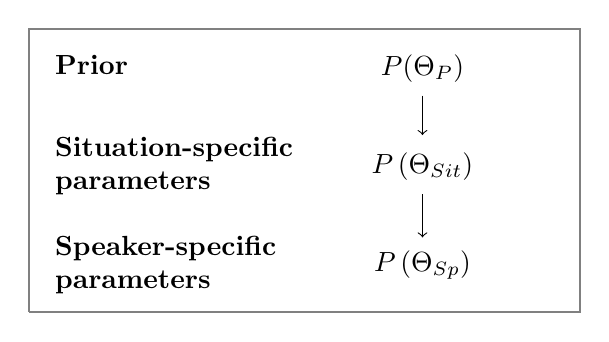
\begin{tikzpicture}
\draw[gray, thick] (0,-0.1) -- (7,-0.1) -- (7,3.5) -- (0,3.5) -- (0,-0.1);
\draw (0, 3.0) node[anchor=west] {\begin{tabular}{l} {\bf Prior} \end{tabular}};
\draw (0, 1.75) node[anchor=west] {\begin{tabular}{l} {\bf Situation-specific} \\ {\bf parameters} \end{tabular}};
\draw (0, 0.5) node[anchor=west] {\begin{tabular}{l} {\bf Speaker-specific} \\ {\bf parameters} \end{tabular}};

\draw (5, 3.0) node {$P(\Theta_P)$};

\draw (5, 1.75) node {$P\left(\Theta_{Sit}\right)$};

\draw (5, 0.5) node {$P\left(\Theta_{Sp}\right)$};


\draw[black,->] (5, 2.65) -- (5, 2.15);


\draw[black ,->] (5, 1.4) -- (5, 0.85);


\end{tikzpicture}
%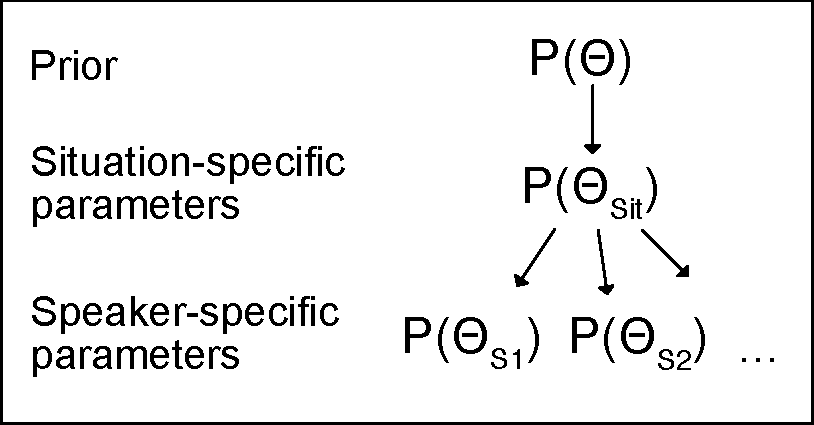
\includegraphics[width=\columnwidth]{plots/model.pdf}
\caption{Hierarchical model of semantic adaptation. Situation-specific parameters $P(\Theta_{Sit})$ depend on prior beliefs $P(\Theta_P)$ and speaker-specific parameters $P(\Theta_{Sp})$ depend on the situation-specific parameters. \label{fig:model}}
\end{figure}



A second possibility would be to cast the model as a mixture model in which overall production parameters are a 
weighted combination of situation-specific and speaker-specific parameters (and potentially other factors). 
Figure~\ref{fig:mixture-model} shows a sketch of a potential mixture model.
According to such a model, listeners would form both situation-specific and speaker-specific
expectations as a result of adaptation and then combine these expectations to their overall expectations. 
Such a model would also predict the smaller effect size in Experiment~1 since it would predict
that the overall production expectations are influenced by the speaker-specific statistics as 
well as the situation-specific statistics and the latter drive the production expectations to be more similar to
an ``average'' speaker. When listeners are exposed to two identical speakers, on the other hand, the 
situation-specific expectations (which are in line with the speaker type of both exposure speakers) 
would reinforce the speaker-specific expectations and therefore lead to a larger adaptation effect. Future experimental work should adjudicate between the hierarchical and the mixture model account.

\begin{figure}
\center
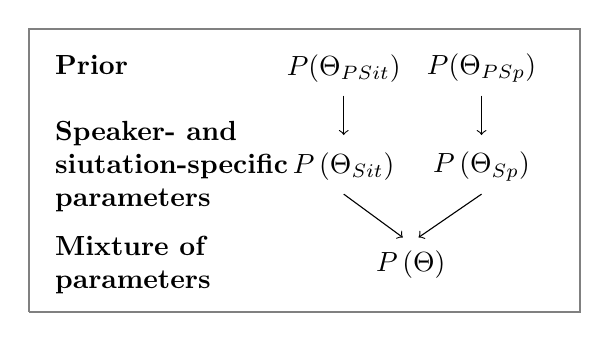
\begin{tikzpicture}
\draw[gray, thick] (0,-0.1) -- (7,-0.1) -- (7,3.5) -- (0,3.5) -- (0,-0.1);
\draw (0, 3.0) node[anchor=west] {\begin{tabular}{l} {\bf Prior} \end{tabular}};
\draw (0, 1.75) node[anchor=west] {\begin{tabular}{l} {\bf  Speaker- and} \\ {\bf siutation-specific} \\ {\bf parameters} \end{tabular}};
\draw (0, 0.5) node[anchor=west] {\begin{tabular}{l} {\bf Mixture of} \\ {\bf parameters} \end{tabular}};

\draw (4, 3.0) node {$P(\Theta_{PSit})$};

\draw (5.75, 3.0) node {$P(\Theta_{PSp})$};


\draw (4, 1.75) node {$P\left(\Theta_{Sit}\right)$};

\draw (5.75, 1.75) node {$P\left(\Theta_{Sp}\right)$};

\draw (4.85, 0.5) node {$P\left(\Theta\right)$};


\draw[black,->] (5.75, 2.65) -- (5.75, 2.15);

\draw[black,->] (4, 2.65) -- (4, 2.15);


\draw[black,->] (5.75, 1.4) -- (4.95, 0.85);
\draw[black,->] (4, 1.4) -- (4.75, 0.85);




\end{tikzpicture}
%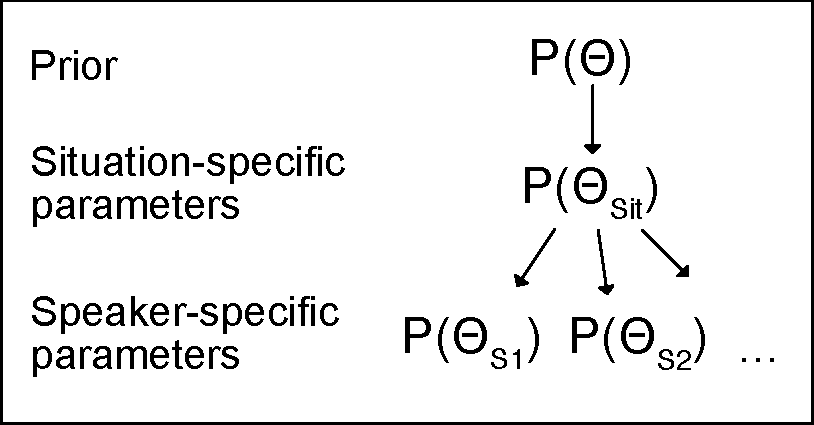
\includegraphics[width=\columnwidth]{plots/model.pdf}
\caption{Mixture model of semantic adaptation. Overall production parameters $P\left(\Theta\right)$ are a weighted combination of situation-specific parameters $P\left(\Theta_{Sit}\right)$ and speaker-specific parameters $P\left(\Theta_{Sp}\right)$ . \label{fig:mixture-model}}
\end{figure}

In conclusion, we presented new experimental results from the domain of uncertainty expressions which suggest that speaker-specific semantic adaptation
is a product of forming speaker-specific expectations and forming expectations about the situation independent of the
speaker.
These results raise a number of interesting questions, most pressingly regarding transfer effects to novel speakers, which 
have been observed in other linguistic domains \egcite{Bradlow2008,Xie2018}. In our experiments, the exposure and test speakers
did not differ. This raises the question about whether and to what extent updated expectations transfer to novel speakers whose similarity to the exposure speaker(s) varies.
Both models sketched above lend themselves well to capturing such transfer effects.
In addition, participants saw very similar visual scenes on each trial. Another potential direction would be to study the 
extent of speaker-specific adaptation when listeners encounter more novel scenes during the test phase to investigate to what extent
listeners form speaker-specific expectations independent of other contextual factors.
Answering these
questions will help disentangle the different adaptation processes and give us a better understanding
of how listeners infer meanings in context.

